% =====================================================================
%  Chapitre 4 -- Entraînement, régularisation et transfert
%  Partie b : régularisation, augmentation, transfert, quiz, TP4
% =====================================================================

\begin{frame}{Régulariser : apprendre le motif, pas le bruit}
\begin{columns}[t]
\begin{column}{0.52\textwidth}
\begin{itemize}
  \item \textbf{Régulariser} = ajouter des contraintes ou du bruit \emph{pendant}
  l'entraînement pour réduire l'écart train/validation.
  \item Objectif : meilleure \textbf{généralisation}, pas meilleure performance
  d'entraînement.
  \item Deux familles : agir sur les \textbf{poids} (weight decay) ou sur
  l'\textbf{information} qui circule (dropout, augmentation).
\end{itemize}
\begin{kbox}[La règle d'or]
Un léger \emph{mieux} sur la validation vaut toujours un \emph{facile} sur
l'entraînement.
\end{kbox}
\end{column}
\begin{column}{0.46\textwidth}
\begin{ebox}[Les cinq outils de ce chapitre]
\begin{enumerate}
  \item Dropout.
  \item Batch normalization.
  \item Weight decay.
  \item Early stopping.
  \item Augmentation de données.
\end{enumerate}
\end{ebox}
\begin{wbox}[À ne pas confondre]
La \emph{batch normalization} normalise \textbf{en interne}, couche par couche ;
la \emph{normalisation des entrées} est faite une fois, avant l'entraînement.
\end{wbox}
\end{column}
\end{columns}
\end{frame}

\begin{frame}{Dropout : éteindre des neurones au hasard}
\begin{columns}[t]
\begin{column}{0.50\textwidth}
\centering
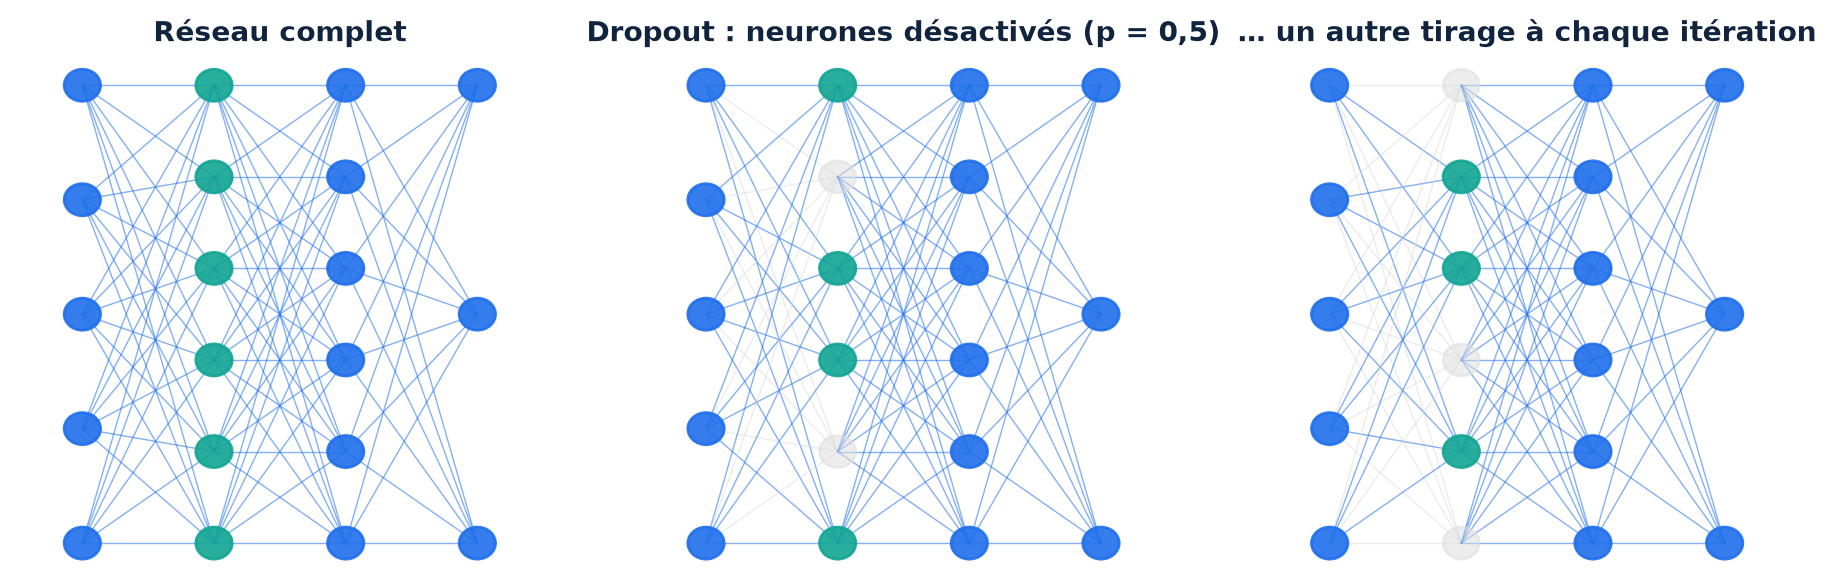
\includegraphics[width=\textwidth]{i02_dropout.png}
\end{column}
\begin{column}{0.46\textwidth}
\begin{itemize}
  \item À chaque itération, on désactive une fraction $p$ des neurones.
  \item Ici $p = 0{,}5$ : la moitié des neurones est mise à zéro.
  \item Le réseau ne peut plus s'appuyer sur un neurone unique : il répartit
  l'information.
\end{itemize}
\begin{kbox}[Effet attendu]
Moins de \emph{co-adaptation} entre neurones $\to$ moins de surapprentissage.
\end{kbox}
\end{column}
\end{columns}
\end{frame}

\begin{frame}{Dropout : ce qui se passe vraiment}
\begin{columns}[t]
\begin{column}{0.50\textwidth}
\begin{ebox}[Sur un petit groupe de 6 neurones]
Avec $p = 0{,}5$, environ \textbf{4 neurones sur 6} restent actifs à une
itération donnée : les deux autres sont éteints \emph{pour cette itération}.
\end{ebox}
\begin{itemize}
  \item La sélection change à \emph{chaque} itération : le réseau n'apprend
  jamais la même sous-architecture.
\end{itemize}
\begin{kbox}[Usage]
Surtout dans les couches \emph{denses} ($p$ de $0{,}3$ à $0{,}5$) ; plus rare
dans les couches convolutives.
\end{kbox}
\end{column}
\begin{column}{0.46\textwidth}
\begin{wbox}[Deux pièges]
\begin{itemize}
  \item Le dropout est actif \emph{seulement} en mode entraînement
  (\py{model.train()}).
  \item À l'évaluation, on repasse en \py{model.eval()} : sinon les prédictions
  deviennent aléatoires.
\end{itemize}
\end{wbox}
\begin{ebox}[En pratique]
Le dropout est un régularisateur \emph{puissant} mais mal dosé il ralentit la
convergence : à introduire quand le surapprentissage est avéré.
\end{ebox}
\end{column}
\end{columns}
\end{frame}

\begin{frame}{Batch normalization : stabiliser les activations}
\begin{columns}[t]
\begin{column}{0.50\textwidth}
\centering
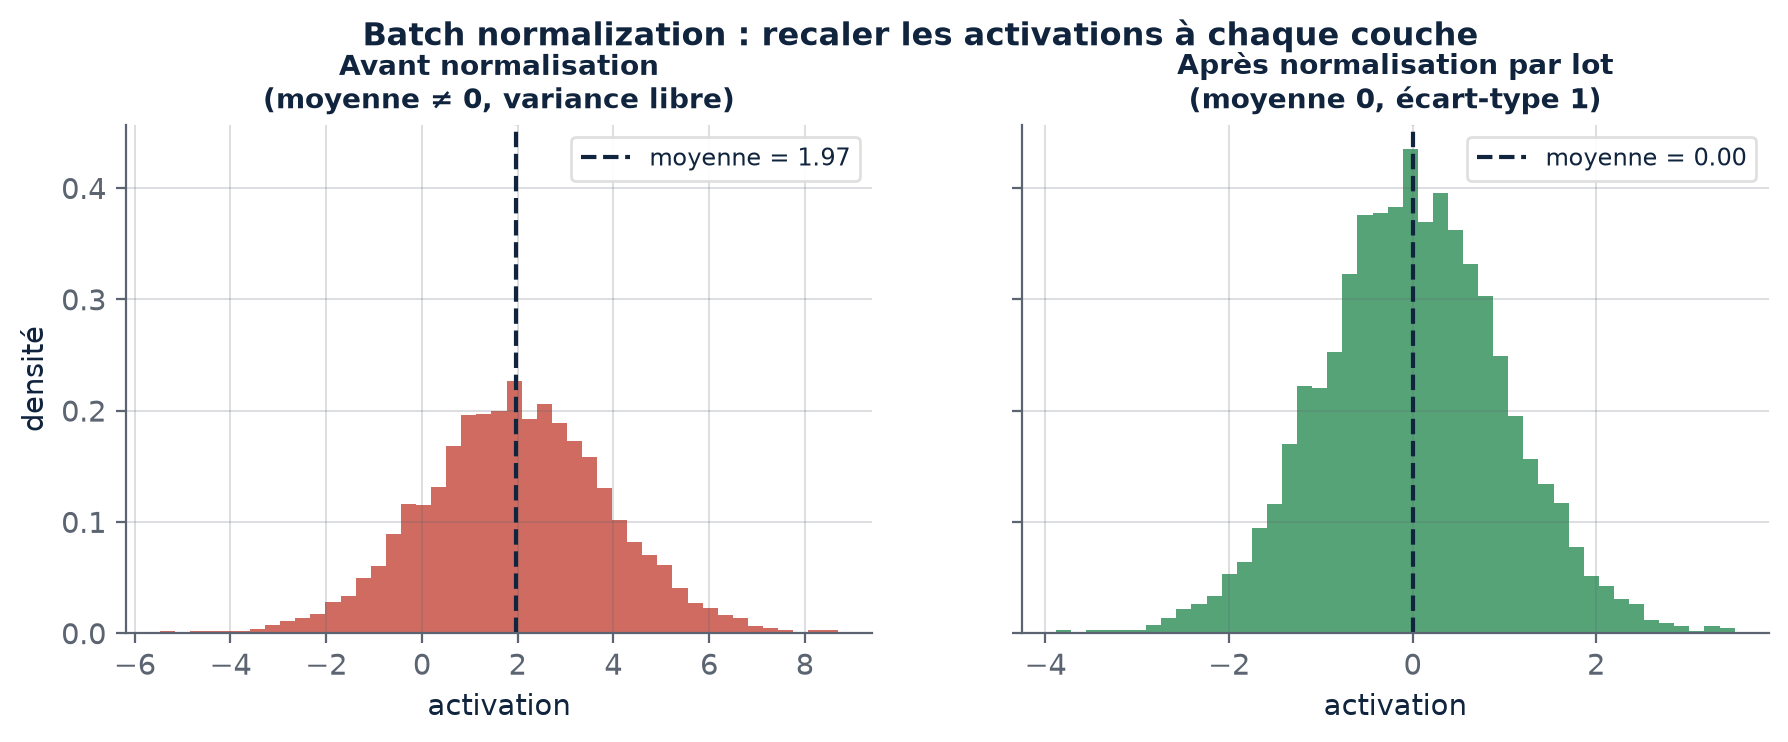
\includegraphics[width=\textwidth]{i03_batchnorm.png}
\end{column}
\begin{column}{0.46\textwidth}
\begin{itemize}
  \item Avant : les activations d'une couche ont une moyenne et un écart-type
  quelconques.
  \item La BN recalcule, sur chaque lot, moyenne et variance, puis ramène les
  activations à une distribution standard.
\end{itemize}
\begin{kbox}[Le résultat]
Après BN, moyenne $\approx 0$ et écart-type $\approx 1$ : les couches suivantes
reçoivent des entrées bien centrées.
\end{kbox}
\end{column}
\end{columns}
\end{frame}

\begin{frame}{Batch normalization : l'effet chiffré}
\begin{columns}[t]
\begin{column}{0.50\textwidth}
\begin{center}
\begin{tabular}{@{}lcc@{}}
\toprule
\textbf{Statistique} & \textbf{Avant BN} & \textbf{Après BN} \\
\midrule
Moyenne & $1{,}974$ & $0{,}0$ \\
Écart-type & $1{,}918$ & $1{,}0$ \\
\bottomrule
\end{tabular}
\end{center}
\begin{kbox}[Lecture]
Les activations, dispersées autour de $1{,}97$, sont ramenées à une moyenne
nulle et une dispersion unité.
\end{kbox}
\end{column}
\begin{column}{0.46\textwidth}
\begin{ebox}[Pourquoi c'est utile]
\begin{itemize}
  \item Entraînement plus stable : gradients mieux conditionnés.
  \item Pas d'apprentissage plus agressifs sans diverger.
  \item Léger effet régularisateur (par le bruit inter-lots).
\end{itemize}
\end{ebox}
\begin{wbox}[Attention évaluation]
En test, la BN utilise des statistiques \emph{cumulées} sur l'entraînement,
pas celles du lot courant.
\end{wbox}
\end{column}
\end{columns}
\end{frame}

\begin{frame}{Weight decay : freiner les grands poids}
\begin{columns}[t]
\begin{column}{0.52\textwidth}
\begin{itemize}
  \item On ajoute au coût une pénalité sur la \emph{taille} des poids :
\end{itemize}
\[
\mathcal{L}_{\text{total}} = \mathcal{L} + \lambda \sum_i w_i^2
\]
\begin{itemize}
  \item $\lambda$ : coefficient de pénalité.
  \item Effet : les poids restent petits, les frontières de décision plus
  \textbf{simples}, donc moins de surapprentissage.
\end{itemize}
\begin{kbox}[Dans PyTorch]
\py{torch.optim.Adam(model.parameters(), lr=1e-3, weight_decay=1e-4)}
\end{kbox}
\end{column}
\begin{column}{0.46\textwidth}
\begin{ebox}[Interprétation]
La pénalité exprime un \emph{a priori} : « à performance égale, préfère le
modèle le plus simple ». C'est le principe du rasoir d'Ockham appliqué aux CNN.
\end{ebox}
\begin{wbox}[Trop de pénalité]
Un $\lambda$ trop grand écrase les poids : le réseau devient trop simple et
\emph{sous-apprend}.
\end{wbox}
\end{column}
\end{columns}
\end{frame}

\begin{frame}{Early stopping : arrêter au bon moment}
\begin{columns}[t]
\begin{column}{0.52\textwidth}
\begin{itemize}
  \item On surveille la perte de \textbf{validation} à chaque époque.
  \item On garde le meilleur modèle et l'on arrête dès qu'elle cesse de
  s'améliorer.
  \item On ne se fie \emph{jamais} à la perte d'entraînement, qui continue
  de baisser.
\end{itemize}
\begin{kbox}[Retour sur l'exemple]
Le minimum de validation était à l'\textbf{époque 5} : c'est là qu'il faut
s'arrêter.
\end{kbox}
\end{column}
\begin{column}{0.46\textwidth}
\begin{ebox}[Deux réglages]
\begin{itemize}
  \item \textbf{Patience} : nombre d'époques tolérées sans progrès.
  \item \textbf{Meilleure époque} : on restaure les poids correspondants.
\end{itemize}
\end{ebox}
\begin{wbox}[Pourquoi c'est la plus rentable]
L'early stopping ne coûte qu'une courbe de validation à surveiller et se
cumule avec tous les autres régularisateurs.
\end{wbox}
\end{column}
\end{columns}
\end{frame}

\begin{frame}{Augmentation de données : multiplier les exemples}
\begin{columns}[t]
\begin{column}{0.50\textwidth}
\centering
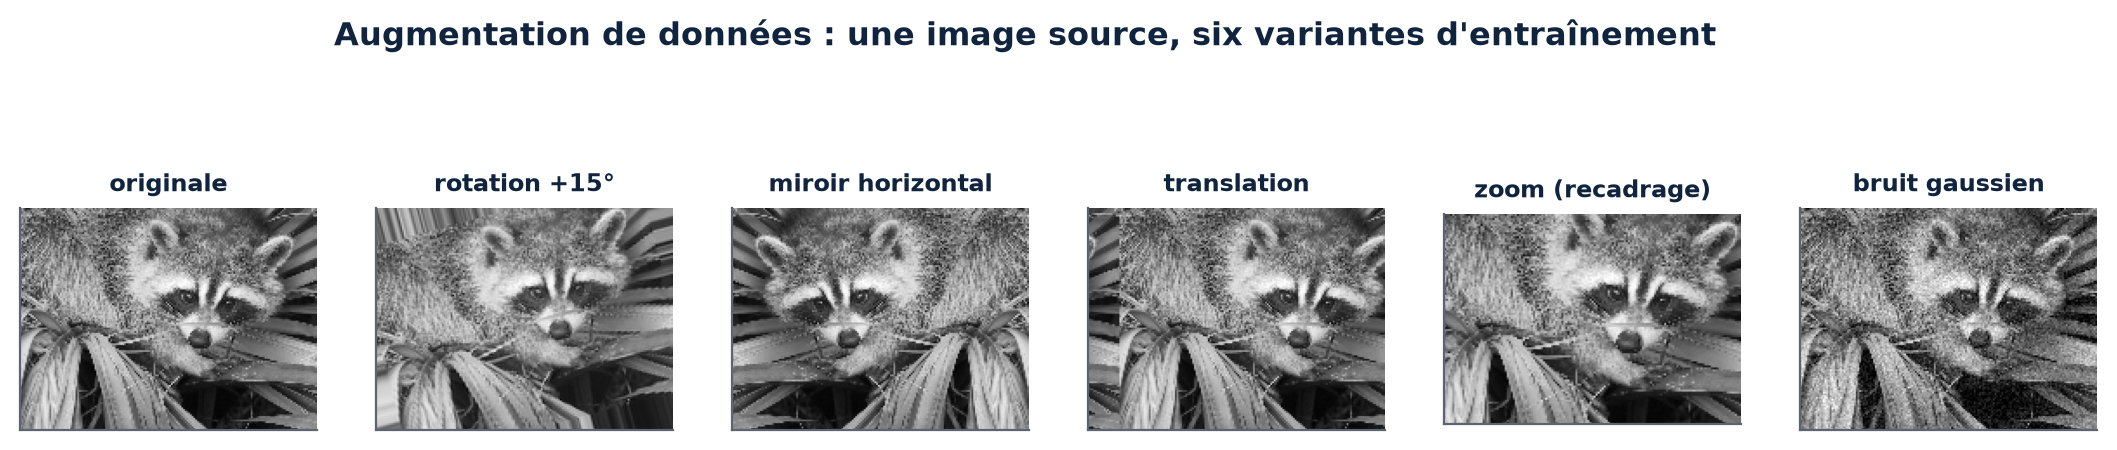
\includegraphics[width=\textwidth]{i04_augmentation.png}
\end{column}
\begin{column}{0.46\textwidth}
\begin{itemize}
  \item On fabrique des variantes \emph{plausibles} de chaque image pour enrichir
  le jeu d'entraînement.
  \item Chaque image originale donne ici \textbf{6 variantes} : le jeu est
  virtuellement multiplié par $6$.
  \item La transformation s'applique \emph{à l'entraînement}, jamais à
  l'évaluation.
\end{itemize}
\begin{kbox}[Motif conservé]
Le contenu de la classe (le chiffre, l'objet) doit rester reconnaissable : on
n'invente pas des exemples impossibles.
\end{kbox}
\end{column}
\end{columns}
\end{frame}

\begin{frame}{Les six variantes d'augmentation}
\begin{columns}[t]
\begin{column}{0.50\textwidth}
\begin{ebox}[Variantes utilisées]
\begin{enumerate}
  \item originelle
  \item rotation $+15^\circ$
  \item miroir horizontal
  \item translation
  \item zoom (recadrage)
  \item bruit gaussien
\end{enumerate}
\end{ebox}
\begin{kbox}[Le principe]
Chaque transformation encode une \emph{invariance} que l'on veut transmettre au
modèle : un chiffre tourné reste le même chiffre.
\end{kbox}
\end{column}
\begin{column}{0.46\textwidth}
\begin{wbox}[Transformations réalistes uniquement]
Un miroir vertical transforme un « 6 » en « 9 » : sur MNIST, les flips
verticaux sont \emph{à éviter}. Toute augmentation doit respecter le sens de la
tâche.
\end{wbox}
\begin{ebox}[En pratique]
Rotation et translation : quasi universelles. Bruit gaussien : utile sur les
capteurs bruités. Le recadrage/zoom : adapté aux photos, plus délicat sur les
formes centrées.
\end{ebox}
\end{column}
\end{columns}
\end{frame}

\begin{frame}{Transfert learning : réutiliser un réseau déjà entraîné}
\begin{columns}[t]
\begin{column}{0.50\textwidth}
\centering
\end{column}
\begin{column}{0.46\textwidth}
\begin{itemize}
  \item Idée : les premières couches d'un CNN apprennent des motifs
  \emph{génériques} (bords, textures) utiles à toutes les tâches visuelles.
  \item On part d'un modèle pré-entraîné et on l'adapte à notre problème.
  \item Rien à réinventer : on profite de ce que d'autres ont appris.
\end{itemize}

\end{column}
\end{columns}
% [fix] figure sortie
% [fix] bloc deplace
\end{frame}
\begin{frame}{Transfert learning : réutiliser un résea… (suite)}
\begin{kbox}[Pourquoi c'est décisif]
Quand notre jeu est petit, le transfert donne souvent de bien meilleurs
résultats qu'un entraînement from scratch. On réentraîne seulement une ou deux
langues.\footnote{\;Le jargon de l'image : un modèle (modèle de base) en haut, un modèle cible en bas.}
\end{kbox}
\end{frame}

\begin{frame}{Transfert learning : réutiliser un réseau déjà entraîné --- la figure}\begin{center}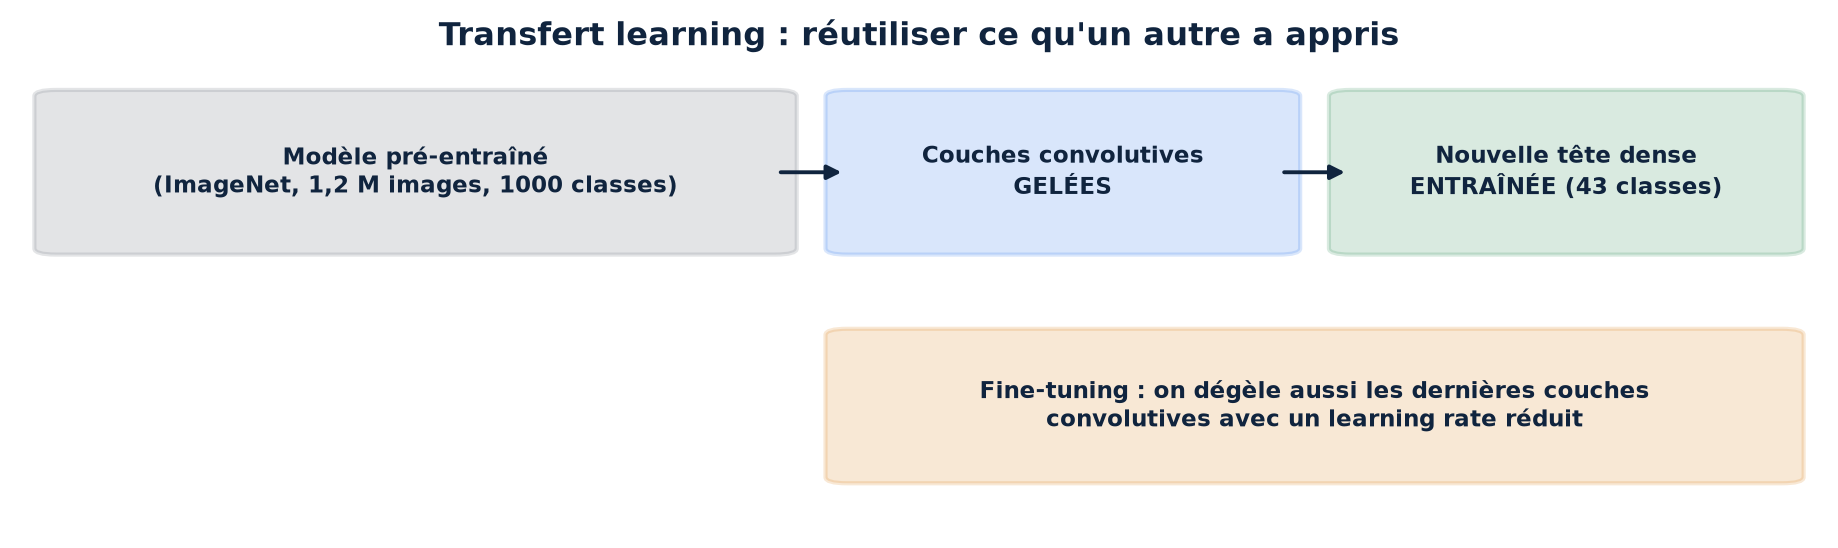
\includegraphics[width=.92\textwidth]{i05_transfert.png}\end{center}\end{frame}

\begin{frame}{Deux façons de transférer}
\begin{columns}[t]
\begin{column}{0.48\textwidth}
\begin{ebox}[Extraction de caractéristiques]
On \textbf{gèle} le réseau pré-entraîné et on n'entraîne qu'une nouvelle
tête de classification.
\begin{itemize}
  \item Très rapide, peu de paramètres à ajuster.
  \item Idéal quand le jeu cible est petit.
\end{itemize}
\end{ebox}
\end{column}
\begin{column}{0.48\textwidth}
\begin{ebox}[Fine-tuning]
On \textbf{dégèle} tout ou partie du réseau et on continue l'entraînement,
avec un pas réduit.
\begin{itemize}
  \item Plus lent, adapte les filtres aux données cibles.
  \item À réserver aux jeux suffisamment grands.
\end{itemize}
\end{ebox}
\end{column}
\end{columns}
\vspace{1mm}
\begin{kbox}[Le réseau de référence : ImageNet]
Le modèle pré-entraîné est presque toujours appris sur \textbf{ImageNet} :
$1{,}2$ \textbf{M} images, \textbf{1\,000} classes. Ces filtres se
\textbf{transfèrent} bien vers d'autres tâches visuelles.
\end{kbox}
\end{frame}

\begin{frame}{Trois erreurs classiques}
\begin{columns}[t]
\begin{column}{0.32\textwidth}
\begin{wbox}[Normalisation oubliée]
On oublie de normaliser les entrées (moyenne/écart-type) ou de mettre le modèle
en \emph{mode entraînement}. Les couches voient des distributions inattendues :
convergence lente ou erratique.
\end{wbox}
\end{column}
\begin{column}{0.32\textwidth}
\begin{wbox}[Fuite de données]
Des exemples de validation (ou de test) se retrouvent dans l'entraînement ; les
scores deviennent trompeusement bons. Ex. : doublons, ou mélange des ensembles
sans graine fixe.
\end{wbox}
\end{column}
\begin{column}{0.32\textwidth}
\begin{wbox}[Déséquilibre de classes]
Une classe très majoritaire écrase les autres : la performance globale est
bonne mais la classe rare est mal reconnue. Remèdes : pondération, sur/sous-échantillonnage.
\end{wbox}
\end{column}
\end{columns}
\vspace{1mm}
\begin{kbox}[Le fil conducteur]
Ces trois erreurs ne sont pas des bugs de code : ce sont des erreurs de
\textbf{méthodologie} d'expérimentation.
\end{kbox}
\end{frame}

\begin{frame}{Quiz}
\begin{columns}[t]
\begin{column}{0.49\textwidth}
\begin{qbox}[Question 1]
Le dropout est activé à l'entraînement. Que se passe-t-il à l'évaluation si
l'on oublie \py{model.eval()} ?
\begin{itemize}
  \item[(a)] Rien \quad (b) Les neurones sont éteints au hasard, les prédictions
  deviennent instables \quad (c) Le réseau devient plus précis
\end{itemize}
\end{qbox}
\begin{qbox}[Question 2]
La batch normalization ramène la moyenne et l'écart-type des activations à
quelles valeurs ?
\begin{itemize}
  \item[(a)] $1$ et $0$ \quad (b) $0$ et $1$ \quad (c) On ne les modifie pas
\end{itemize}
\end{qbox}
\end{column}
\begin{column}{0.49\textwidth}
\begin{qbox}[Question 3]
Sur MNIST, pourquoi la rotation de $+15^\circ$ enrichit-elle les données, alors
qu'un miroir vertical est dangereux ?
\end{qbox}
\begin{qbox}[Question 4]
Je dispose de 500 photos, toutes d'une seule classe d'objet. Vaut-il mieux
entraîner from scratch ou faire du transfert ?
\begin{itemize}
  \item[(a)] From scratch \quad (b) Transfert (extraction de caractéristiques)
  \quad (c) Aucune différence
\end{itemize}
\end{qbox}
\end{column}
\end{columns}


% [fix] bloc deplace
% [fix] bloc deplace
\end{frame}
\begin{frame}{Quiz (suite)}
\begin{qbox}[Question 5]
La perte de validation minimal se situe à l'époque 5 et remonte après. Que
faut-il faire ?

\end{qbox}
\end{frame}
\begin{frame}{Quiz (suite)}
\begin{itemize}
  \item[(a)] Continuer jusqu'à la perte nulle \quad (b) Arrêter / early stopping
  à l'époque 5 \quad (c) Augmenter le pas d'apprentissage
\end{itemize}
\end{frame}

\begin{frame}{Réponses}
\begin{solbox}[Réponses --- à ne regarder qu'après avoir répondu]
\textbf{1.} (b) : la sélection aléatoire est appliquée par erreur à l'inférence,
les prédictions deviennent erratiques. \quad
\textbf{2.} (b) : après BN, moyenne $0$ et écart-type $1$. \quad
\textbf{3.} Une rotation change légèrement l'orientation du chiffre mais le
laisse reconnaissable ; un miroir vertical transforme un « 6 » en « 9 », donc
change la classe. \quad
\textbf{4.} (b) : petit jeu et peu de données, l'extraction de caractéristiques
sur un modèle pré-entraîné (ImageNet) est de loin la meilleure option. \quad
\textbf{5.} (b) : le minimum de validation indique le bon moment pour arrêter
(ici l'époque 5) et restaurer ces poids.
\end{solbox}
\end{frame}

\begin{frame}{À retenir}
\begin{columns}[t]
\begin{column}{0.50\textwidth}
\begin{kbox}[Les cinq idées clés]
\begin{enumerate}
  \item Entraîner = répéter prédire, coût, corriger, sur des lots.
  \item Le pas d'apprentissage fait tout : trop petit, trop grand ou adapté.
  \item Lire les courbes : creuser l'écart train/validation = surapprentissage.
  \item Régulariser : dropout, BN, weight decay, early stopping.
  \item Transfert : réutiliser ImageNet plutôt que repartir de zéro.
\end{enumerate}
\end{kbox}
\end{column}
\begin{column}{0.46\textwidth}
\begin{ebox}[Les chiffres du chapitre]
Trop petit $0{,}001$ / adapté $0{,}05$ / trop grand $0{,}9$ ; dropout
$p = 0{,}5$ ; BN : moyenne $0$, écart-type $1$ ; arrêt à l'époque $5$ ;
ImageNet : $1{,}2$ M images, $1\,000$ classes.
\end{ebox}
\begin{wbox}[La leçon]
Une bonne architecture ne sauve pas un mauvais entraînement ; c'est la
méthode --- régulariser, augmenter, transférer --- qui fait la généralisation.
\end{wbox}
\end{column}
\end{columns}
\end{frame}

\begin{frame}{Passons à la pratique}
\begin{columns}[t]
\begin{column}{0.50\textwidth}
\begin{abox}[TP4 : régularisation et augmentation]
\textbf{Notebook :} \file{notebooks/TP4\_regularisation\_augmentation.ipynb}
\begin{itemize}
  \item Ajouter du dropout et du weight decay à un CNN.
  \item Insérer une batch normalization et observer la stabilité.
  \item Augmenter les données (rotations, translations, flips, bruit).
  \item Comparer les courbes avec et sans régularisation.
\end{itemize}
\end{abox}
\end{column}
\begin{column}{0.46\textwidth}
\begin{kbox}[Ce que vous manipulerez]
\begin{itemize}
  \item \py{torch.nn.Dropout}, \py{torch.nn.BatchNorm2d}.
  \item \py{weight_decay} dans l'optimiseur.
  \item \py{torchvision.transforms} pour l'augmentation.
  \item Un « early stopping » maison.
\end{itemize}
\end{kbox}
\begin{ebox}[Objectif]
Reproduire, sur MNIST et un sous-ensemble de CIFAR-10, le saut de généralisation
qu'apporte la régularisation.
\end{ebox}
\end{column}
\end{columns}
\end{frame}